% CECI EST UN FICHIER DE MODÈLE LATEX POUR LES ARTICLES INCLUS DANS
% *Anthology of Computers and the Humanities*. AJOUTEZ L’OPTION
% 'final' LORS DE LA CRÉATION DE LA VERSION FINALE DE L’ARTICLE. 
% NE PAS modifier la classe du document
\documentclass[final,fra]{anthology-ch} % pour la version finale
%\documentclass[fra]{anthology-ch}         % pour la soumission

% CHARGER LES PACKAGES LaTeX
\usepackage{booktabs}
\usepackage{graphicx}

%Update

% Insertion de common.latex en enlevant babel
% https://github.com/jgm/pandoc-templates/blob/master/common.latex



\usepackage{longtable,booktabs,array}
\usepackage{calc} % for calculating minipage widths
% Correct order of tables after \paragraph or \subparagraph
\usepackage{etoolbox}
\usepackage{graphicx}
\usepackage{seqsplit}
\usepackage{microtype}


%/ common.latex inclusion

% AJOUTEZ vos propres packages avec \usepackage{}

% TITRE DE LA SOUMISSION
% Remplacez ceci par le titre de votre soumission
\title{Agentivité épistémique et recherche assistée par IA: un système
de recommandation transparent pour la recherche informationnelle
exploratoire}

% INFORMATIONS SUR LES AUTEURS ET LES AFFILIATIONS
% Pour chaque auteur, utilisez une nouvelle commande \author, avec
% les numéros entre crochets indiquant les affiliations correspondantes
% (section suivante) et l’ORCID-ID pour chaque auteur.  
\author[1]{Alexia Schneider}[
  orcid=0009-0000-0651-9792,
  email=alexia.schneider@umontreal.ca
]
\author[1]{Marcello Vitali-Rosati}[
  orcid=0000-0001-6424-3229,
  email=marcello.vitali.rosati@umontreal.ca
]
\author[1]{Pierre Lévy}[
  orcid=0000-0003-1599-221X,
  email=
]
\affiliation{1}{Université de Montréal}


% MOTS-CLÉS
% Fournissez un ou plusieurs mots-clés séparés par des virgules
% en utilisant la commande suivante

\keywords[fra]{système de recommandation, recherche d'information,
           recherche exploratoire, ieml}
\keywords[eng]{recommender system, AI-research assistant, exploratory search practices}

% MÉTADONNÉES DE LA PUBLICATION
% Ces champs seront remplis lors de la publication ; 
% ils peuvent être laissés par défaut lors de la soumission
\pubyear{2026}
\pubvolume{4}
\pagestart{55}
\pageend{62}
\conferencename{Actes de la Conférence Humanistica}
\conferenceeditors{Serena Crespi, Simon Gabay, Martin Grandjean, Ariane Pinche, Marie Puren et Léa Saint-Raymond}
\doi{10.63744/qHjD0KEilhGB}
\customhead{}


\addbibresource{bibliography.bib}

%%%%%%%%%%%%%%%%%%%%%%%%%%%%%%%%%%%%%%%%%%%%%%%%%%%%%%%%%%%%%%%%%%%%%%%%%%%
% DÉBUT DU TEXTE
\paperorder{7}
\begin{document}

\maketitle

\begin{abstract}
Information retrieval tools in academic contexts filter and rank what
researchers read and cite, thereby influencing scientific innovation and
the citation dynamics that shape research. Current ``AI research
assistants'' rely on a natural language querying strategy interpreted by
a large language model ; this paradigm, which appears to attract the
majority of information retrieval resources today, raises questions
about the epistemological impact of interpretations performed by tools
whose black-box effect is well-documented. This paper presents a
recommender system appended to the specialized scientific search engine
Isidore, tool designed as a concrete alternative to natural language
querying. First, we will present the functionalities of the recommender
system developed in this project: constructing a query through iterative
interactions involving terms and definitions using the IEML language;
comparing result lists displayed side-by-side from the user-constructed
query and the same query ``augmented'' by an LLM. Second, we will
present the evaluation of the semantic parsing into IEML performed by an
LLM on a corpus of 360 terms, as well as the results of a small sample
user study.
\end{abstract}

\vspace{1cm}
\section{Introduction : le problème de la recherche assistée par IA opaque}\label{introduction-le-probluxe8me-de-la-recherche-assistuxe9e-par-ia-opaque}

Les systèmes de recommandation (SR) intégrés aux moteurs de recherche
scientifiques influencent ce que les chercheur·e·s voient, lisent et
citent. Pourtant, ces systèmes rendent rarement explicites les
stratégies de recherche d'information (RI) à l'origne des articles
présentés. En conséquence, les SR reposent fréquemment sur des métriques
non sémantiques telles que le nombre de citations, renforçant des
mécanismes de concentration des citations, également connus sous le nom
de \emph{Matthew's effect} \autocite{mertonMatthewEffectScience1968}.
D'autres systèmes dépendent fortement des interactions passées et
enregistrées des utilisateur·ice·s
\autocite{kosterSerendipitousRecommendationBased2014}, créant des
risques de bulles de filtres \autocite{pariserFilterBubble2012} et
de biais de confirmation dans le travail scientifique
\autocite{underwoodTheorizingResearchPractices2014}.

Le glissement actuel vers des ``assistants IA'' conversationnels,
reposant sur un paradigme générique de requêtes en langue naturelle
analysées par des grands modèles de langue (GML), rend de plus en plus
pressantes les questions de modélisation alternative, d'interprétabilité
et d'agentivité épistémique que les Humanités Numériques adressent
\autocite{goodladEditorsIntroductionHumanities2023,vitali-rosatiManifestePourEtudes2025a}.
Si les mécanismes derrière les recommandations générées par l'IA
demeurent opaques, les chercheur·e·s perdent la capacité d'évaluer de
manière critique la façon dont la pertinence est construite.

Notre question de recherche principale est la suivante : quelle
alternative aux assistants de recherche IA peut être conçue afin de
mettre en avant des connexions inattendues de manière explicable et
transparente pour l'utilisateur·ice ? Pour donner plus de perspective à
cette question : qu'est-ce qu'une comparaison directe entre une
ontologie symbolique et une recherche sémantique fondée sur les GML peut
révéler sur leurs modèles épistémiques sous-jacents ?

Ancrée dans les propositions de
\autocite{druckerPerformativeMaterialityTheoretical2013}, l'outil
développé pour répondre à ces questions se veut un révélateur
d'incertitudes et d'interprétations subjectives afin de sensibiliser à
la littératie en IA. Nous présentons ainsi \texttt{IEML-RS}, un SR
reposant sur un processus collaboratif et itératif de construction de
requêtes pour une phase de recherche d'information exploratoire
réflechie et transparente. Nous présentons dans un deuxième temps
l'évaluation de l'outil à travers les résultats d'une étude utilisateur
et sur l'évaluation technique du parsing sémantique en IEML produit par
des GML.

\section{Contexte et état de l'art}\label{contexte-et-uxe9tat-de-lart}

Les outils récents de recherche assistée par IA fonctionnent sur
l'utilisation de GML pour l'expansion de requêtes, le classement de
pertinence et la synthèse automatisée, à toutes ces étapes, les
``choix'' du modèle sont probabilistes; l'hypothèse distributionnelle
\autocite{firthStudiesLinguisticAnalysis1962,harrisDistributionalStructure1981}
au coeur de ces algorithmes et de l'IA connexionniste suppose que les
fréquences de cooccurrences d'unités syntaxiques permettent à
elles-seules de reconstruire la langue et indirectement, ses aspects
sémantiques.

Bien qu'efficace pour la production de texte, cette approche renforce
implicitement les connexions et les chemins sémantiques les plus
probables, ce qui dans le cas de la publication académique risque de
privilégier une littérature déjà citée et de réduire l'espace
épistémique de la découverte
\autocite{nielsenGlobalCitationInequality2021,vargaNarrowingLiteratureUse2022}.
Les évaluations des assistants de recherche fondés sur l'IA montrent
également une opacité persistante, un rappel inégal et une tendance à
survaloriser les travaux dominants ou fortement cités
\autocite{pattersonWhichAITools2025,archambaultEvaluationCuttingEdgeAI2024}.
Comme le soutient
\autocite{tayReproducibilityInterpretabilityAcademic2025}, le manque de
transparence des systèmes contemporains de RI fondés sur les GML
complique la capacité des utilisateur·ice·s à évaluer de manière
critique les résultats, soulignant la nécessité d'approches mettant au
premier plan l'explicabilité et l'agentivité des utilisateur·ice·s.

En tant qu'objectif, la sérendipité et la recherche exploratoire
proposent un paradigme alternatif dans la construction des SR. Des
travaux fondateurs conceptualisent la sérendipité comme un processus
itératif mené par l'utilisateur·ice, de ``\emph{berrypicking}'', dans
lequel les requêtes évoluent par variantes au fil d'un parcours non
linéaire alternant rencontres de documents et d'idées
\autocite{batesDesignBrowsingBerrypicking1989,erdelezInformationEncounteringIts1999}.
Des modèles ultérieurs soulignent la nature évaluative et définie par
l'utilisateur·ice de la sérendipité : une découverte ne devient
``trouvaille'' qu'a posteriori, lorsqu'on est à même de réinterprèter sa
pertinence
\autocite{makriComingInformationSerendipitously2012}.
Des études empiriques en contexte académique confirment le rôle de la
sérendipité dans la diversification des pratiques de lecture et le
développement d'expertises transdisciplinaires
\autocite{fosterSerendipityInformationSeeking2003}. Des exemples
d'appropriation détournée des fonctionnalités principales des moteurs de
recherche suggèrent que les pratiques effectives de recherche restent
encore largement non cartographiées et plus diverses que ne le laissent
entendre les pratiques guidées actuelles de RI
\autocite{dumasprimbaultNaviguerDansSavoirs2023}. Pourtant, la majorité
des SR demeurent orientée vers la personnalisation et l'interrogation en
langue naturelle, visant une RI intuitive plutôt qu'une exploration
étendue ou un soutien à l'engagement des chercheur·se·s dans la
complexité de leurs propres investigations.

Quelques outils scientifiques tentent de réintroduire l'exploration dans
la RI pour la recherche scientifique. \texttt{Bridger}
\autocite{portenoyBurstingScientificFilter2022} expose les
chercheur·se·s à des auteur·ice·s extérieur·e·s à leurs réseaux
intellectuels habituels afin de favoriser le décloisonnement
disciplinaire. \texttt{VITALITY}
\autocite{narechaniaVITALITYPromotingSerendipitous2022} propose une
approche de revue de littérature fondée sur la visualisation, mais
repose sur des corpus fortement sélectionnés et prétraités. D'autres
projets, tels que \texttt{STAK}
\autocite{martinSTAKSerendipitousTool2017}, s'est inspiré des
affordances matérielles des bibliothèques physiques en tentant de
recréer des environnements de navigation spatialisés.

Les alternatives aux approches fondées sur les GML incluent les graphes de 
connaissances et les ontologies du Web sémantique. Au sein des représentations 
sémantiques symboliques, OWL et RDF sont des formalismes bien établis, et 
l'Information Economy MetaLanguage (IEML) \cite{levySemanticComputingIEML2023} 
bien que moins connu, offre une alternative flexible pertinente pour l'exploration 
de champs conceptuel. IEML est un langage d'explicitation sémantique fondée sur 
une logique de composition à partir d'unités sémantiques prédéfinies. Les 
dimensions sémantiques constituent une ontologie fixe de neuf aspects 
(thème/processus, qui, quoi, à qui, par quels moyens, quand, où, pourquoi, 
comment) permettant des définitions flexibles et heuristiques de tout concept 
dans une structure aisément intelligible et manipulable.

\begin{table}[h]
    \centering
    \begin{tabular}{ll}
    \textbf{Mot-clé} & \textbf{Conteuse} \\
    Thème       & communication \\
    Qui         & $\sim$ féminin conteur \\
    Quoi        & récit \\
    À qui       & \\
    Par quoi    & \\
    Quand       & \\
    Où          & \\
    Pourquoi    & \\
    Comment     & \\
    \end{tabular}
    \caption{Décomposition sémantique avec IEML.}
    \label{tab:ieml}
\end{table}


Le Tableau \ref{tab:ieml} offre une visualisation explicite d'une traduction attendue
en IEML du concept de ``conteuse'' : tous les aspects ne sont pas
obligatoirement remplis et la flexion d'une valeur peut être signifiée
par le symbole \texttt{\textasciitilde{}}.

Alors que les GML sont de plus en plus utilisés pour des tâches
complexes de \emph{parsing} sémantique non structuré, des évaluations
récentes montrent qu'ils demeurent peu fiables pour les langages
sémantiques structurés. Par exemple, les modèles d'OpenAI ont obtenu de
faibles performances dans la génération d'Abstract Meaning
Representation (AMR), même avec quelques exemples dans le prompt
\autocite{ettingerYouAreExpert2023}. Cela renforce la nécessité de
cadres sémantiques explicites et interprétables dans la RI scientifique.
Contrairement à la représentation canonique unique de l'AMR, IEML
propose une décomposition sémantique flexible et ajustable par
l'utilisateur·ice, susceptible de soutenir la variation exploratoire.
Cependant, aucun travail antérieur n'a examiné la traduction automatique
en IEML ni son intégration dans des systèmes de recommandation.

Ensemble, ces lacunes motivent la nécessité de SR transparents et ancrés
dans une logique interprétative, qui préservent le contrôle des
utilisateur·ice·s, soutiennent la variation exploratoire et rendent
visibles les différences épistémiques entre approches symboliques et
connexionnistes. L'outil \texttt{IEML-RS} contribue à cet espace en
offrant une comparaison double, côte à côte, entre une recherche fondée
sur l'ontologie et une recherche sémantique fondée sur les GML dans un
contexte réel de découverte scientifique.

\section{IEML-RS}\label{ieml-rs}

Notre système de recommandation d'articles est une extension du
navigateur Firefox en Javascript qui dialogue avec le moteur de
recherche \href{https://isidore.science}{Isidore} pour les SHS
francophones via son site web (en extrayant les métadonnées de l'article
de départ) et son API (fonction de recherche d'articles par mots-clés).
L'utilisateur·ice commence sur une page d'article dont les métadonnées
sont extraites. Les mots-clés dont une traduction validée manuellement
existe sont présentés en bleus, les autres sont en oranges.
% \documentclass{article}
% \usepackage[utf8]{inputenc}
% \usepackage[T1]{fontenc}
% \usepackage[french]{babel}
% \usepackage{graphicx}
% \usepackage{hyperref}


\noindent
\begin{minipage}{0.475\textwidth}
\centering
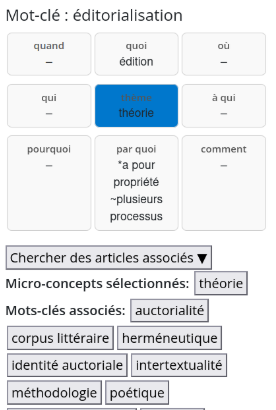
\includegraphics[width=.65\linewidth, alt={Sélectionner une cellule affiche tous les mots-clés employant en IEML le même concept}]{mot-cle-visualisation.png}
\captionof{figure}{Sélectionner une cellule affiche tous les mots-clés employant en IEML le même concept.}
\label{fig:motcle}
\end{minipage}%
\hspace{0.5cm} 
\begin{minipage}{0.475\textwidth}
La sélection d'un mot-clé fait apparaître sa forme de grille et sa traduction en IEML, soit sous forme validée (mots-clés bleus), soit sous forme de grille à corriger (mots-clés oranges). La sélection d'une cellule de la grille fait apparaître tous les mots-clés utilisant le même concept. Dans l'exemple de la figure~\ref{fig:motcle}, la sélection de la facette thème ``théorie'' du mot-clé ``éditorialisation'' révèle que les mots-clés ``auctorialité'', ``corpus littéraire'', ``herméneutique'' etc. sont aussi traduits avec ``théorie'' dans leur grille IEML. En proposant une conceptualisation simple sous la forme d'une grille qu'il est possible à son tour de remplir, les utilisateur·ice·s non familier·e·s avec IEML peuvent aisément établir des connexions sémantiques complexes tout en apprenant à utiliser le SR.
\end{minipage}
% \vspace{0.5pt}

\noindent
\begin{minipage}{0.475\textwidth}
\centering
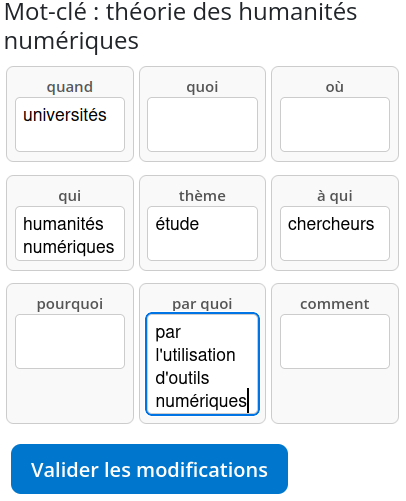
\includegraphics[width=.65\linewidth, alt={Traduction automatique du mot-clé ``théorie des humanités numériques'' en IEML par le modèle gemma-3n-E4B-it}]{grille-Traduction.png}
\captionof{figure}{Traduction automatique du mot-clé ``théorie des humanités numériques'' en IEML par le modèle gemma-3n-E4B-it.}
\label{fig:traduction}
\end{minipage}%
\hspace{0.5cm} 
\begin{minipage}{0.475\textwidth}

L'un des intérêt saillant du système de recommandation repose dans la portée reflexive du
processus de construction de la requête, processus qui émane de la
matrice de décomposition sémantique en IEML (voir tab.~\ref{tab:ieml})
mais aussi de la traduction automatique en IEML d'un mot-clé générée par
\texttt{gemma-3n-E4B-it} (voir \hyperref[trad-ieml]{figure}). Correction
et validation par l'utilisateur·ice de la grille pré-remplie par GML
impliquent une forme de mise en dialogue réflexive non seulement avec le
concept sélectionné mais aussi, indirectement, avec le GML qui a produit
la proposition de traduction.

\end{minipage}
\vspace{1em}
\protect\phantomsection\label{trad-ieml}{}

L'utilisateur·ice construit sa requête sur la base des concepts et
mots-clés sélectionnés dans cette phase itérative d'exploration (la
sélection est visible en vert sur la \hyperref[panels]{figure}). Le
lancement d'une recherche d'articles laisse voir les panels listant les
résultats des requêtes permettant ainsi une visualisation de l'impact
habituellement invisible de la médiation par les GML dans les pratiques
de recherche (\hyperref[panels]{{[}panels{]}}).

\begin{figure}
\centering
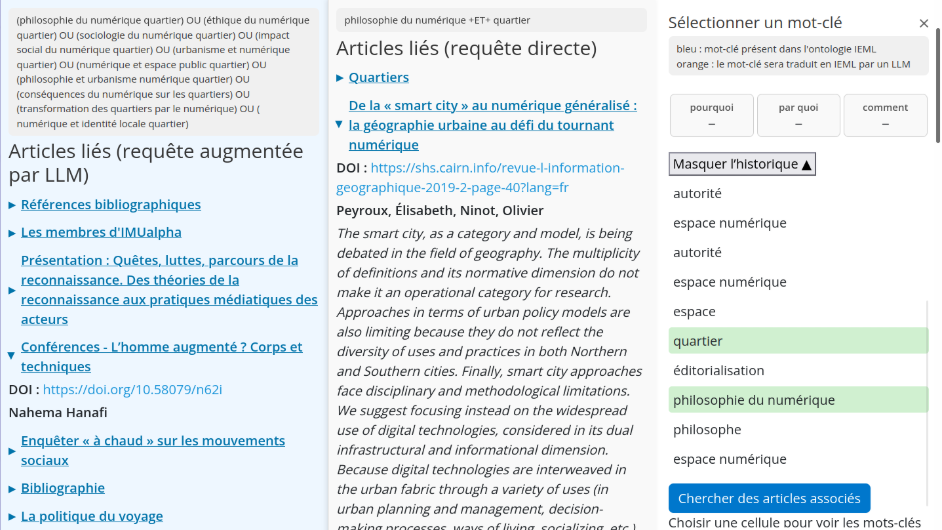
\includegraphics[width=.9\linewidth,alt={Comparaison côte à côte des articles extraits de la requête construite par l'utilisateur·ice, puis à partir d'une augmentation de cette requête enrichie par LLM. Le bloc supérieur gris indique la requête envoyée à l'API d'Isidore.}]{etape6-affichage-Articles2.png}
\caption{Comparaison côte à côte des articles extraits de la requête
construite par l'utilisateur·ice, puis à partir d'une augmentation de
cette requête enrichie par LLM. Le bloc supérieur gris indique la
requête envoyée à l'API d'Isidore.}
\label{panels}
\end{figure}

\section{Évaluations}\label{uxe9valuations}

\subsection{Évaluation de GML pour le parsing sémantique en
IEML}\label{uxe9valuation-de-gml-pour-le-parsing-suxe9mantique-en-ieml}

L'une des principales fonctionnalités du SR est la traduction
collaborative homme-machine en IEML proposée pour des mots-clés absents
de la base de données validée manuellement des concepts en IEML. Cette
fonctionnalité repose sur une traduction proposée par un GML que
l'utilisateur·ice peut corriger (\hyperref[trad-ieml]{{[}trad-ieml{]}}).
Ces mots-clés corrigés et validés sont ensuite ajoutés à la base de
données IEML, conformément à la notion d'intelligence collective
affirmée par le concepteur d'IEML
\autocite{levyCollectiveIntelligenceMankinds1997}.

\begin{table}[h]
\centering
\begin{tabular}{llll}
\toprule
\textbf{Model} & \textbf{BLEU avg} & \textbf{Cosine avg} & \textbf{Avg} \\
\midrule
noRAG llama\_fewshot & 5.6e-2 & 0.515 & 0.286 \\
llama\_zeroshot      & 1.3e-2 & 0.514 & 0.263 \\
gemma\_zeroshot      & 1.6e-2 & 0.479 & 0.248 \\
openai\_zeroshot     & 1.6e-2 & 0.493 & 0.255 \\
llama\_fewshot       & 2.2e-2 & 0.555 & 0.289 \\
gemma\_fewshot       & 2.0e-2 & 0.491 & 0.255 \\
openai\_fewshot      & 1.7e-2 & 0.498 & 0.257 \\
\bottomrule
\end{tabular}
\caption{Résultat des traductions en IEML par GML de 360 mots-clés.}
\label{tab:resultats}
\end{table}

\protect\phantomsection\label{rag-eval}{}

Pour cette tâche, nous avons évalué trois GML propriétaires
(\href{https://huggingface.co/openai/gpt-oss-20b}{\texttt{GPT-oss-20B}}, 
\href{https://huggingface.co/meta-llama/Meta-Llama-3-70B-Instruct}{\texttt{\seqsplit{Meta-Llama-3-70B-Instruct-Turbo}}}, 
\href{https://huggingface.co/google/gemma-3n-E4B-it}{\texttt{Gemma-3n-E4V-it}})
sur leur capacité à traduire 360 mots-clés en IEML partant d'un système
de génération augmentée de récupération (\emph{RAG}) avec un prompt
contenant 60 exemples et une récupération de 20 mots sélectionnés dans
le dictionnaire IEML (\textasciitilde3 000 entrées). Les scores
quantitatifs montrent des gains négligeables avec les exemples
contextuels (\hyperref[rag-eval]{{[}rag-eval{]}}), et l'analyse
qualitative a confirmé que les modèles échouent à reproduire les
contraintes structurelles d'IEML. Les mesures de distances sémantiques
(cosine et score BLEU) ne conviennent que partiellement à l'évaluation
de la traduction; la comparaison de vecteurs ne rend pas compte de
l'intérêt de la concaténation de concepts sémantiques possiblement
éloignés mais pertinents dans une traduction en IEML. Cela confirme les
résultats de \autocite{ettingerYouAreExpert2023} sur les limites des GML
pour le \emph{parsing} sémantique structuré, et souligne l'importance de
la validation humaine pour ce type de tâche. Ce résultat oriente nos
perspectives vers de futurs designs de SR intégrant les retours et
interprétations humaines, deux processus cognitifs fondamentaux de la
découverte informationnelle fortuite
\autocite{makriComingInformationSerendipitously2012}.

\subsection{Étude utilisateur}\label{uxe9tude-utilisateur}

\subsubsection{Méthodologie}\label{muxe9thodologie}

Après l'installation et une démonstration de l'ensemble des
fonctionnalités du SR, six utilisateur·ice·s volontaires ont été
observé·e·s lors d'une session de 10 minutes d'interaction avec le
plugiciel, suivie d'un entretien de 15 minutes couvrant les
fonctionnalités et aspects centraux : ergonomie, utilité, navigation par
mots-clés, traduction en IEML, recherche d'articles et comparaison des
panels de listes d'articles extraits.

Les utilisateur·ice·s étaient six doctorant·e·s en humanités numériques
et connaissaient tous les développeur·se·s. Les auteur·ice·s
reconnaissent que ces deux éléments constituent des biais importants de
cette étude et en limitent la portée analytique.

\section{Résultats et discussion}\label{ruxe9sultats-et-discussion}

Les observations issues de l'expérience indiquent que tous les
participant·e·s ont extrait des articles via le SR, suggérant que
l'outil a facilité l'accès à une littérature auparavant inconnue, y
compris pour celles et ceux qui ne recourent pas habituellement à la
recherche par mots-clés. Bien que tous les utilisateur·ice·s aient
formulé plusieurs requêtes et comparé les listes d'articles à des degrés
divers, un seul s'est engagé de manière équivalente dans les deux
étapes. Tous sauf un ont corrigé les traductions générées par les LLM,
et une participante les a annotées plutôt que remplacées, indiquant que
des productions de faible qualité peuvent susciter une posture
dialogique et collaborative vis-à-vis des tâches sémantiques. De telles
traductions imparfaites semblent favoriser la réflexivité dans
l'articulation de concepts sémantiquement riches et soutenir
l'appropriation de l'outil par l'utilisateur·ice. Étant donné le nombre
limité de mots-clés prétraduits (420 au moment de la rédaction), les
utilisateur·ice·s ont fréquemment rencontré des concepts ``non
traduits''; loin de constituer une simple contrainte, cette lacune
représente une opportunité de renforcer l'agentivité des
utilisateur·ice·s en les invitant à formuler el·eux-mêmes les
correspondances conceptuelles manquantes en IEML et à participer à
l'appropriation du SR.

Les participant·e·s ont recommandé diverses améliorations fonctionnelles
et ajustements UX, mais de nombreuses limites semblent résolubles par
une intégration directe à Isidore (par exemple : maintien de l'état de
session, fiches de métadonnées complètes, distinction plus claire entre
la construction de requêtes et la récupération de documents, et
réduction de la latence causée par les appels d'API en chaîne). Les
forces et limites du SR développé seront détaillées lors de la
conférence.

\section{Perspectives}\label{perspectives}

À notre connaissance, cet outil constitue la première application de
construction de requêtes impliquant une conceptualisation sémantique
réalisée de manière collaborative par un humain et un LLM. Nous tenons
que les SR peuvent être des outils critiques qui exposent, plutôt que
dissimulent, les différences de modélisation en amont de la RI
(ontologie vs hypothèse distributionnelle). Dans cette perspective, le
travail amorcé tant lors du développement de notre RS que lors de son
évaluation laisse voir que les pratiques de recherche informationnelle
demeurent variées et qu'il y a encore une place pour la recherche
réflexive en contexte scientifique. De futurs travaux pourraient mettre
à profit cette construction itérative d'une requête dans un contexte
exploratoire pour valoriser et permettre à l'utilisateur·ice de définir
plus clairement ses intentions, intentionalités floues notamment
observées dans les usages d'interaction en langue naturelle avec les GML
\autocite{subramonyamBridgingGulfEnvisioning2024}.


\printbibliography



% Vous pouvez inclure une annexe en utilisant la commande suivante
%\appendix

%\section{Première section de l’annexe} \label{appdx:first}


\end{document}